\newcommand{\erassistant}{ErAssistant~}

\chapter{ПРОБЛЕМАТИКА РАЗРАБОТКИ\\ МУЛЬТИСИНХРОННЫХ УСТРОЙСТВ}

В данном разделе будут рассмотрены проблемы и особенности построение устройств


В этом разделе будут описаны проблемы, возникающие в процессе разработки мультисихронного проекта, то есть устройства, в котором имеют место пересечения клоковых доменов или доменов синхрочастоты (CDC).

\section{Домен синхрочастоты}
Домен синхрочастоты представляет собой ту часть проекта, которая тактируется одной или несколькими синхрочастотами, причем все эти синхрочастоты должны иметь постоянные сдвиги фазы. Если в какой-либо части проекта имеется синхрочастота или инвертированная синхрочастота, или синхрочастота, полученная из исходной путем деления на 2, то такая часть проекта считается клоковым доменом с одной синхрочастотой. Если же домены имеют синхрочастоты с переменной фазой и соотношениями времени, то такие домены считают доменами с различными синхрочастотами. 

На Рисунке \ref{fig:clock-domain} показано, что проект имеет единственный домен синхрочастоты, потому что синхрочастота divClk --- есть деленная на два частота генератора синхронизации Clk.

\begin{figure}[h!]
	\centering
	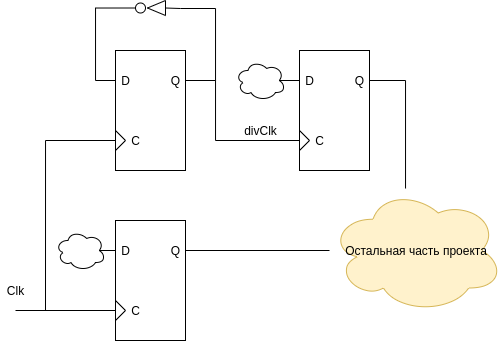
\includegraphics[width=0.6\linewidth]{course-scheme/images/clock-domain}
	\caption{Схема с одним доменом синхрочастоты}
	\label{fig:clock-domain}
\end{figure}


На Рисунке \ref{fig:multiclock-domain} показано несколько синхрочастот от различных источников. Ту часть проекта, которая управляется этими синхрочастотами, называют доменами синхрочастоты, и сигналы, осуществляющие передачу импульсов между этими асинхронными доменами синхрочастоты, называют путями пересечения домена синхрочастоты. Сигнал DA считают асинхронным сигналом в домене синхрочастоты, так как между генератором синхронизации A (clkA) и генератором синхронизации B (ClkB) не существуют постоянные соотношения фазы и времени.

\begin{figure}[h!]
	\centering
	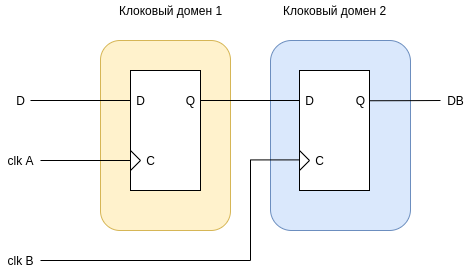
\includegraphics[width=0.7\linewidth]{course-scheme/images/multiclock-domain}
	\caption{Путь домена синхрочастоты}
	\label{fig:multiclock-domain}
\end{figure}


\section{Основные принципы}

При разработке ультисинхрочастотных проектов следует уделять особое внимание стабильности сигнала. Когда сигнал пересекает домен синхрочастоты, то он появляется в новом домене синхрочастоты как асинхронный сигнал и должен быть засинхронизирован.

Синхронизация предотвращает в новом домене синхрочастоты метастабильное состояние первого запоминающего элемента схемы (триггера), и это позволяет в новом домене работать уже со стабильным сигналом.

\textit{Метастабильность} --- это неспособность триггера достигнуть известного состояния в определенный момент времени. Когда триггер входит в метастабильное состояние, то невозможно предсказать ни уровень выходного напряжения элемента, ни период времени, за который этот выход перейдет к правильному уровню напряжения. 

В течение этого переходного времени выход триггера будет находиться на некотором промежуточном уровне напряжения или колебаться и может передать этот недопустимый уровень сигнала со своего выхода к другим триггерам схемы.

\section{Решение проблемы метастабильности}

С целью решения проблемы метастабильности применяются каскады стабилизирующих триггеров, включенных последовательно. Рассмотрим это решение.


Простейший синхронизатор представляет собой два триггера, включенных последовательно без какой-либо комбинационной схемы между ними. Такая схема проекта гарантирует, что первый триггер выходит из своего метастабильного состояния, и его выход переходит в устойчивое состояние перед тем, как второй триггер сохраняет его. Необходимо также разместить эти триггеры, насколько возможно, ближе друг к другу для того, чтобы гарантировать наименьшую расфазировку тактовых сигналов между ними. 

Другой тип ячейки синхронизатора представляет собой два близко расположенных триггера без какой-либо комбинационной логики между ними. Для того чтобы синхронизация работала должным образом, сигнал, пересекающий домен синхрочастоты, должен проследовать от триггера в домене синхрочастоты источника сигнала к первому триггеру синхронизатора, не пройдя через комбинационную логику.

Синхронизацию в домене называют привязкой входного сигнала к тактовой частоте
домена, т. е. все изменения этого сигнала в домене будут происходить по фронту или срезу
тактового сигнала домена, а не родительского тактового сигнала. На Рисунке \ref{fig:sync-triggers}) приведена схема традиционного синхронизатора из
двух триггеров (сдвиговый регистр) для одиночного сигнала. Схема синхронизации приведена на Рисунке \ref {fig:sync-scheme}.

\begin{figure}[h!]
	\centering
	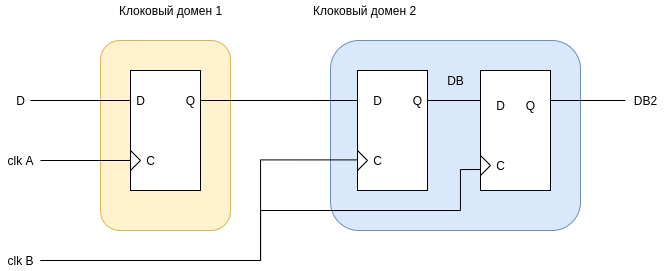
\includegraphics[width=0.7\linewidth]{course-scheme/images/sync-triggers}
	\caption{Триггеры синхронизации}
	\label{fig:sync-triggers}
\end{figure}

\begin{figure}[h!]
	\centering
	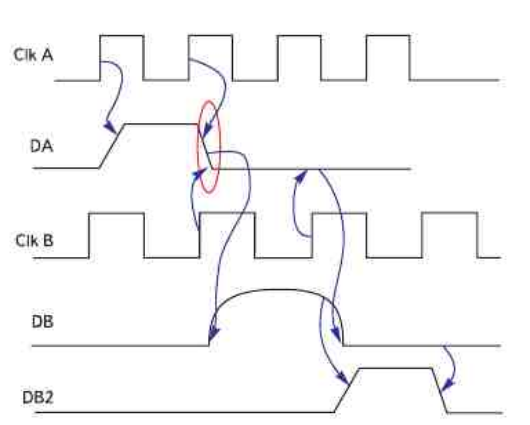
\includegraphics[width=0.5\linewidth]{course-scheme/images/sync-scheme}
	\caption{Схема синхронизации сигнала}
	\label{fig:sync-scheme}
\end{figure}
%\clearpage
%\vspace{2ex}

Данный способ борьбы с метастабильностью будет в дальнейшем использован при разработке узла ресихронизации данных.

\section{Асинхронная очередь}

Во многих проектах необходимо передавать из одного домена в другой не только несколько одиночных сигналов, но и сигналы типа шин: шины данных, адреса и шины управления.

В этих задачах активно используются буферы типа FIFO и специальные протоколы для процедуры установления связи. Особенно полезной оказывается асинхронная очередь, позволяющая производить запись и чтение по синхросигналам двух клоковых доменов.
Данная схема позволяет быстро и удобно передавать данные в реальном времени между двумя разными областями синхронизации.

На Рисунке \ref{fig:async-fifo} приведена схема использования двухпорторой оперативной памяти, позволяющей осуществлять передачу данных между частями устройства, использующими синхросигналы разной частоты.

\begin{figure}[h!]
	\centering
	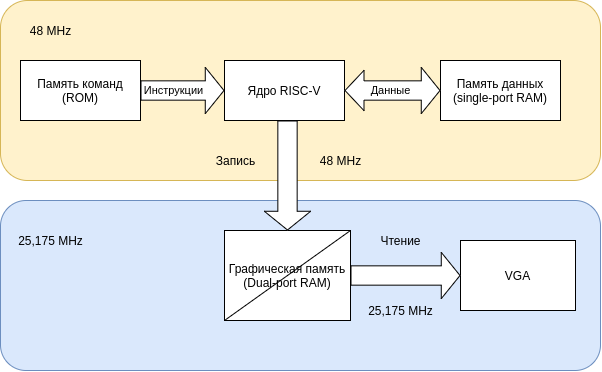
\includegraphics[width=0.7\linewidth]{course-scheme/images/dual-port-ram}
	\caption{Двухпортовая оперативная память}
	\label{fig:async-fifo}
\end{figure}

Двухпортовая память с независимыми тактовыми сигналами --- аппаратный блок, используемый в современных FPGA и в технологических библиотеках для заказных микросхем. Чтение и запись производится совершенно независимо через два отдельных порта.

Единственным ограничением является одновременное обращение на запись и чтение по одному и тому же адресу памяти --- оно может привести к неопределенному результату. На основе такого блока памяти зачастую создается модуль FIFO, который позволяет с одной стороны записывать данные из одного тактового домена, а с другой — забирать в другой тактовый домен. Заодно логика FIFO следит за тем, чтобы не происходило обращения к одной и той же ячейке памяти.

Данный узел работает по следующему принципу. 
\begin{enumerate}
	\item Источник данных загружает данные в асинхронную очередь. Тактирование производится по тактовому сигналу источника данных.
	\item Потребитель данных считывает данные из асинхронной очереди в исходном порядке. Тактирование производится по тактовому сигналу потребителя данных. 
\end{enumerate}



